\section{Cálculo de Pi mediante MPI y PThreads.}

Paralelizamos dividiendo la carga de trabajo primero entre procesos y luego en cada proceso
entre hebras, de forma equitativa.

Ejecutamos con \texttt{ppi.sh}.

\begin{figure}[H]
    \centering
    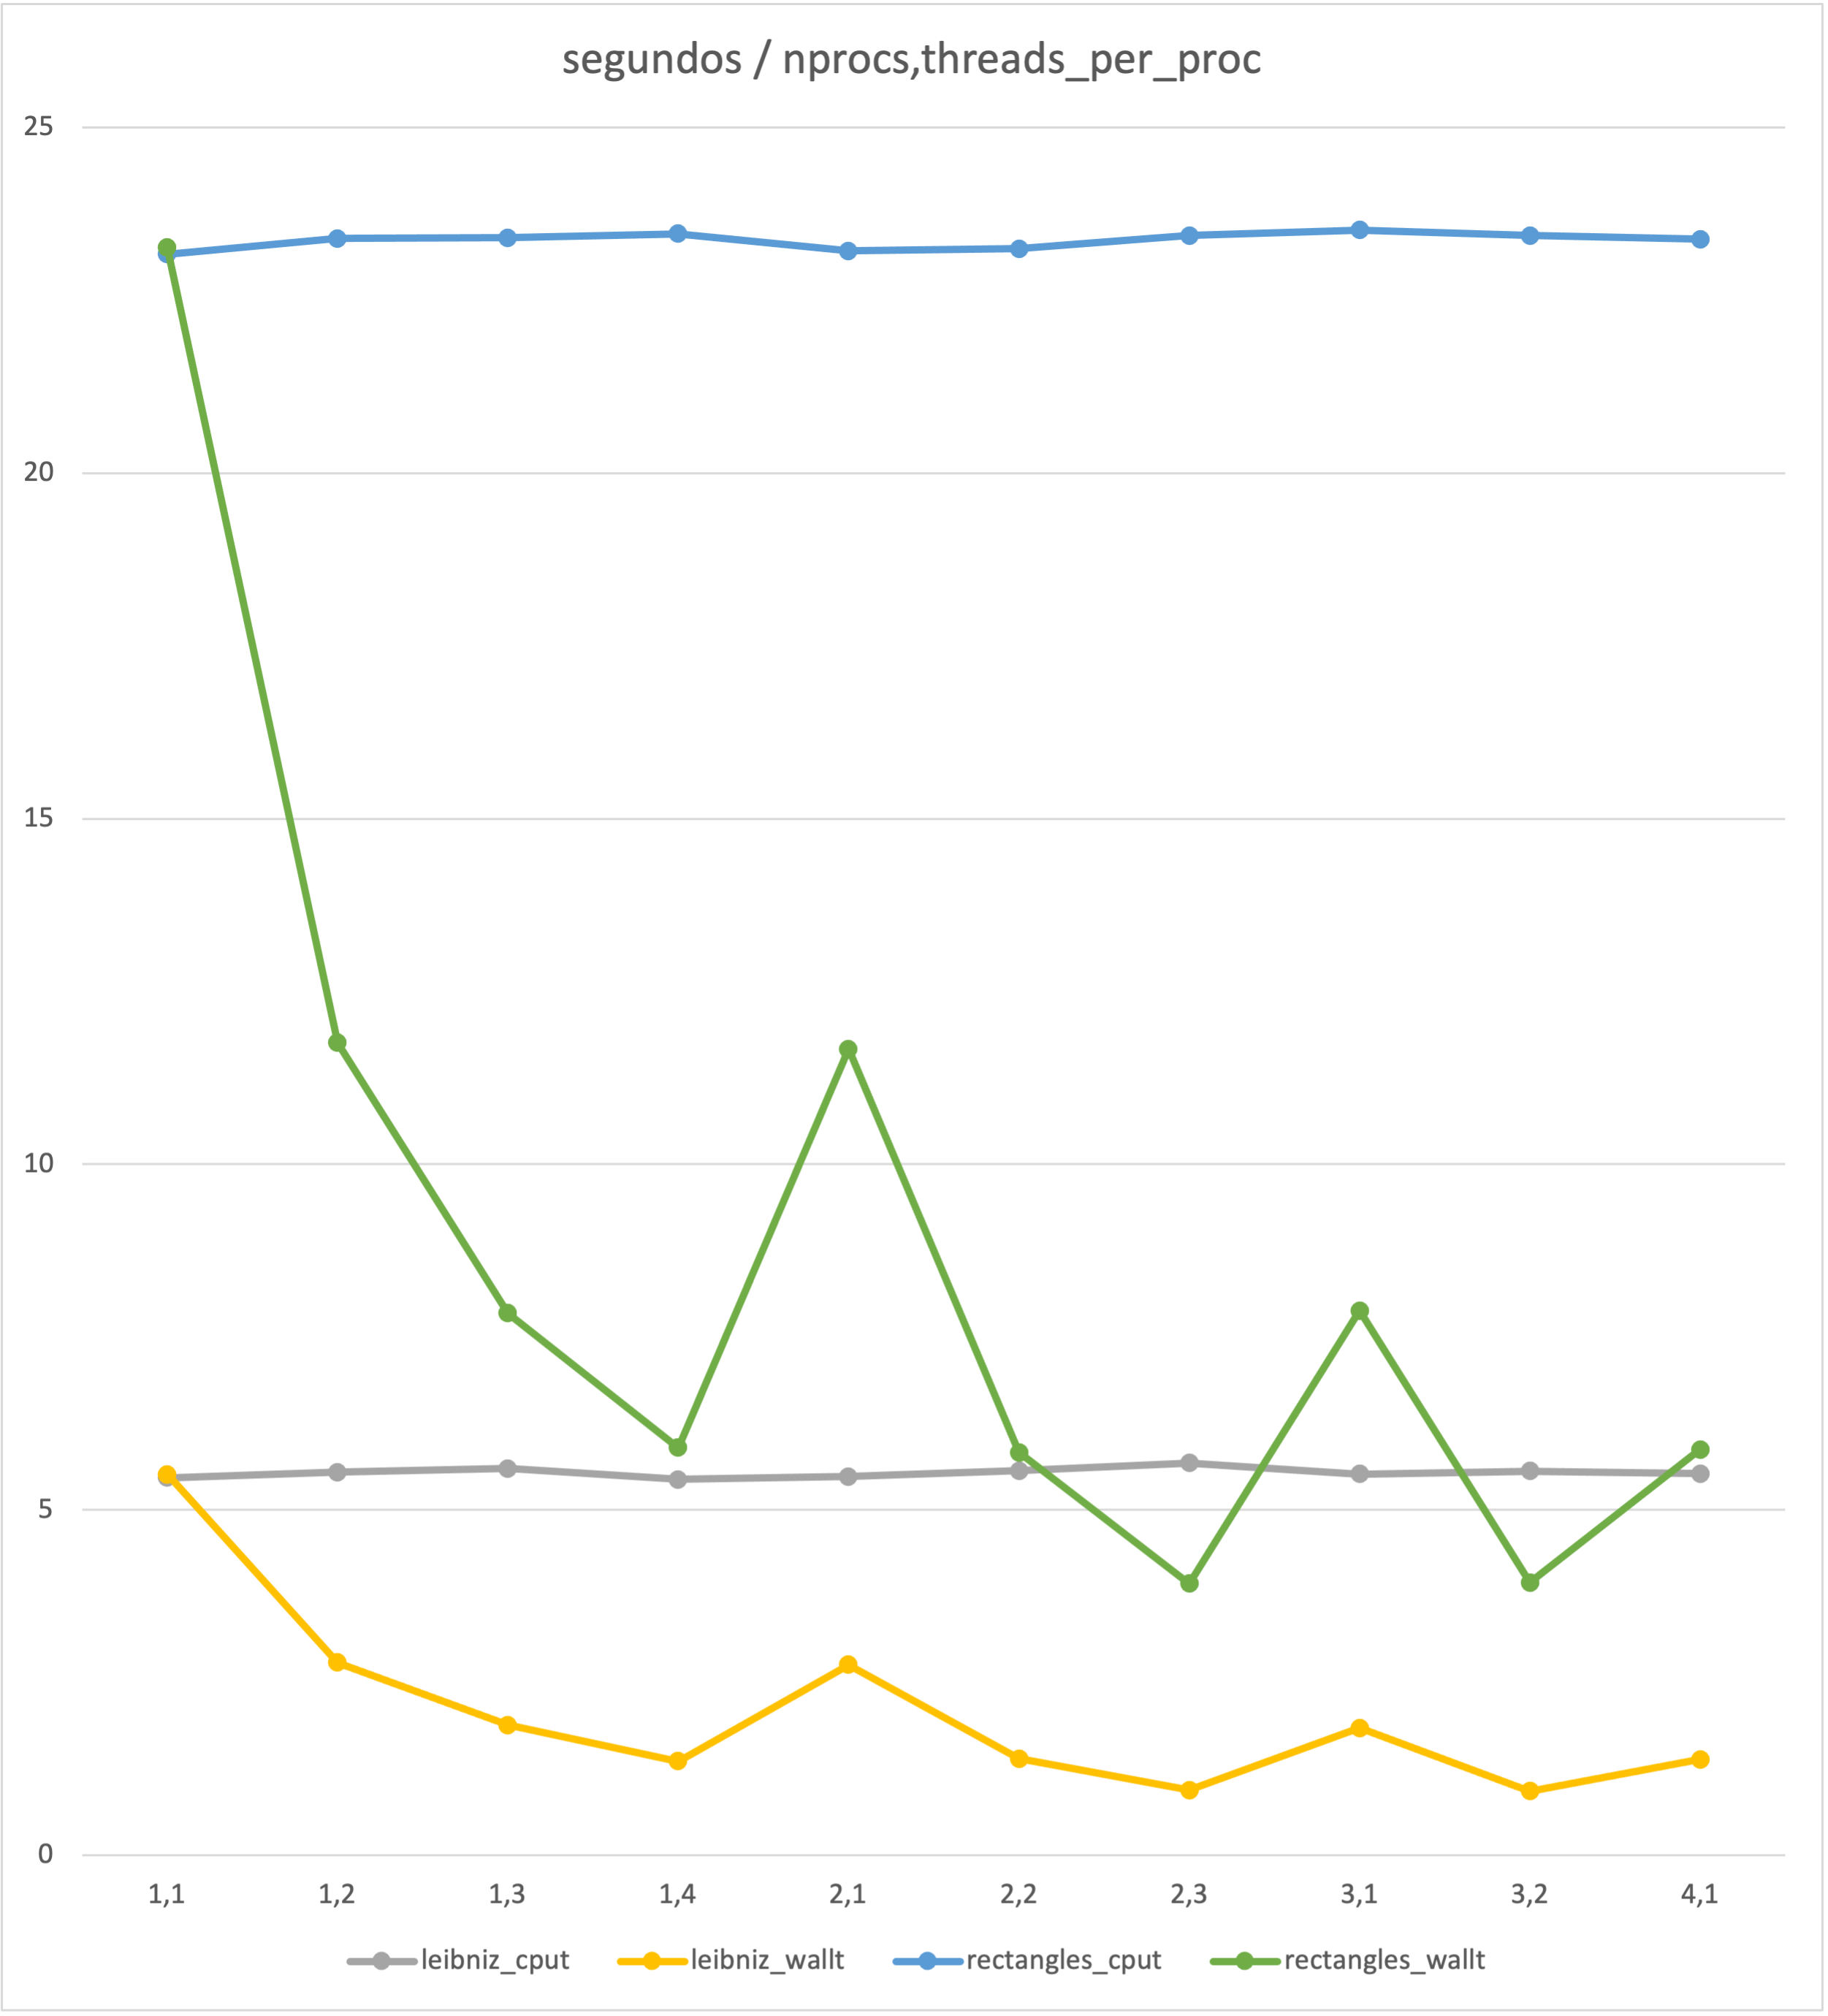
\includegraphics[width=\textwidth]{ej4.png}
    \caption{Relación segundos / número de procesos,hebras por proceso. Podemos observar cómo son resultados
    similares cuando tenemos un mismo número de unidades de ejecución, independientemente de su naturaleza.
    Esto se debe a que el número de mensajes intercambiados es mínimo y nuestros algoritmos no se ven afectados
    por el tipo de acceso a memoria.}
\end{figure}